%% 
%% Copyright 2019-2021 Elsevier Ltd
%% 
%% This file is part of the 'CAS Bundle'.
%% --------------------------------------
%% 
%% It may be distributed under the conditions of the LaTeX Project Public
%% License, either version 1.2 of this license or (at your option) any
%% later version.  The latest version of this license is in
%%    http://www.latex-project.org/lppl.txt
%% and version 1.2 or later is part of all distributions of LaTeX
%% version 1999/12/01 or later.
%% 
%% The list of all files belonging to the 'CAS Bundle' is
%% given in the file `manifest.txt'.
%% 
%% Template article for cas-sc documentclass for 
%% single column output.
\PassOptionsToPackage{table,xcdraw}{xcolor}
\documentclass[a4paper,fleqn]{cas-sc}

% If the frontmatter runs over more than one page
% use the longmktitle option.

%\documentclass[a4paper,fleqn,longmktitle]{cas-sc}

\usepackage[numbers]{natbib}
%\usepackage[authoryear]{natbib}
%\usepackage[authoryear,longnamesfirst]{natbib}
\let\printorcid\relax % Remove ORCID footnote

%%%packages added by the author
\usepackage{lipsum}
\usepackage{graphicx}
\usepackage{subcaption}
\usepackage[flushleft]{threeparttable}
\usepackage{amssymb}


%%%Author macros
\def\tsc#1{\csdef{#1}{\textsc{\lowercase{#1}}\xspace}}
\tsc{WGM}
\tsc{QE}
\newcommand{\mytitle}{Fault Diagnostics of a Reboiler in a Chlorine Dioxide Generation Plant using MLP}
%%%

% Uncomment and use as if needed
%\newtheorem{theorem}{Theorem}
%\newtheorem{lemma}[theorem]{Lemma}
%\newdefinition{rmk}{Remark}
%\newproof{pf}{Proof}
%\newproof{pot}{Proof of Theorem \ref{thm}}

\begin{document}
	\let\WriteBookmarks\relax
	\def\floatpagepagefraction{1}
	\def\textpagefraction{.001}
	
	% Short title
	\shorttitle{\mytitle}    
	
	% Short author
	\shortauthors{R.S. Queiroz et al.}  
	
	% Main title of the paper
	\title [mode = title]{\mytitle}  
	
	% Title footnote mark
	% eg: \tnotemark[1]
	%\tnotemark[1] 
	
	% Title footnote 1.
	% eg: \tnotetext[1]{Title footnote text}
	%\tnotetext[1]{This document is one of the results of a research project funded by Shell Brasil, SENAI CIMATEC, ANP, and EMBRAPII.} 
	
	% First author
	%
	% Options: Use if required
	% eg: \author[1,3]{Author Name}[type=editor,
	%       style=chinese,
	%       auid=000,
	%       bioid=1,
	%       prefix=Sir,
	%       orcid=0000-0000-0000-0000,
	%       facebook=<facebook id>,
	%       twitter=<twitter id>,
	%       linkedin=<linkedin id>,
	%       gplus=<gplus id>]
	
	\author[1,2]{Rafael S. Queiroz}
	\cormark[1] % Corresponding author indication
	%\fnmark[<footnote mark no>] % Footnote of the first author
	\ead{rafaelq@ufba.br} % Email id of the first author
	%\ead[url]{} % URL of the first author
	
	% Credit authorship
	% eg: \credit{Conceptualization of this study, Methodology, Software}
	\credit{Conceptualization, Methodology, Software, Validation, Formal analysis, Investigation, Writing - Original Draft}
	
	% Address/affiliation
	\affiliation[1]{organization={Department of Mechatronics,
			Federal University of Bahia (UFBA)},
		addressline={R. Prof. Aristídes Novis, 2}, 
		city={Salvador},
		%          citysep={}, % Uncomment if no comma needed between city and postcode
		postcode={40210-630}, 
		state={Bahia},
		country={Brazil}}
	
	% Address/affiliation
	\affiliation[2]{organization={SENAI CIMATEC},
		addressline={Av. Orlando Gomes, 1845}, 
		city={Salvador},
		%          citysep={}, % Uncomment if no comma needed between city and postcode
		postcode={41650-010}, 
		state={Bahia},
		country={Brazil}}
	
	\affiliation[3]{organization={University of California (UCLA)},
		addressline={405 Hilgard Avenue}, 
		city={Los Angeles},
		%          citysep={}, % Uncomment if no comma needed between city and postcode
		postcode={90095}, 
		state={California},
		country={USA}}
	
	\author[3]{Enrique Andres López Droguett}
	%\fnmark[2] % Footnote of the second author
	\ead{eald@ucla.edu} % Email id of the second author
	%\ead[url]{} % URL of the second author
	\credit{Conceptualization, Methodology, Validation, Investigation} % Credit authorship
	
	\author[1,2]{Herman A. Lepikson}
	\ead{herman.lepikson@fieb.org.br}
	\credit{Writing - Review \& Editing, Supervision} % Credit authorship
	
	% Corresponding author text
	\cortext[1]{Corresponding author}
	
	% Footnote text
	%\fntext[1]{}
	
	% For a title note without a number/mark
	%\nonumnote{}
	
	% Here goes the abstract
	\begin{abstract}
	 A neural network is designed to perform the fault diagnosis of a reboiler in a chlorine dioxide generation plant. The dataset of 41,539 acquisition records from 8 sensors is preprocessed and divided into training, validation and test sets. The network, composed of 2 layers -- a hidden one with 32 neurons and an output one with 2 neurons -- achieves an accuracy of 99.61\% in the test set and an area under the ROC curve of 99.98\%, proving to be an excellent tool for diagnosing failures of the studied equipment.
	\end{abstract}
	
	% Use if graphical abstract is present
	%\begin{graphicalabstract}
	%\includegraphics{}
	%\end{graphicalabstract}
	
	% Research highlights
	%\begin{highlights}
	%\item
	%\item
	%\item
	%\end{highlights}
	
	% Keywords
	% Each keyword is seperated by \sep
	\begin{keywords}
		Fault diagnosis \sep Multilayer perceptron \sep Neural networks \sep Reboiler
	\end{keywords}
	
	\maketitle
	
	% Main text
	\section{Introduction}\label{sec:intro}
	
	The reboiler in a chlorine dioxide generation process in a cellulose plant, shown schematically in Figure \ref{fig:cellulose-plant}, presents a degradation problem due to scaling build up with potential tube rupture. 
	
	\begin{figure}[h]
		\centering
		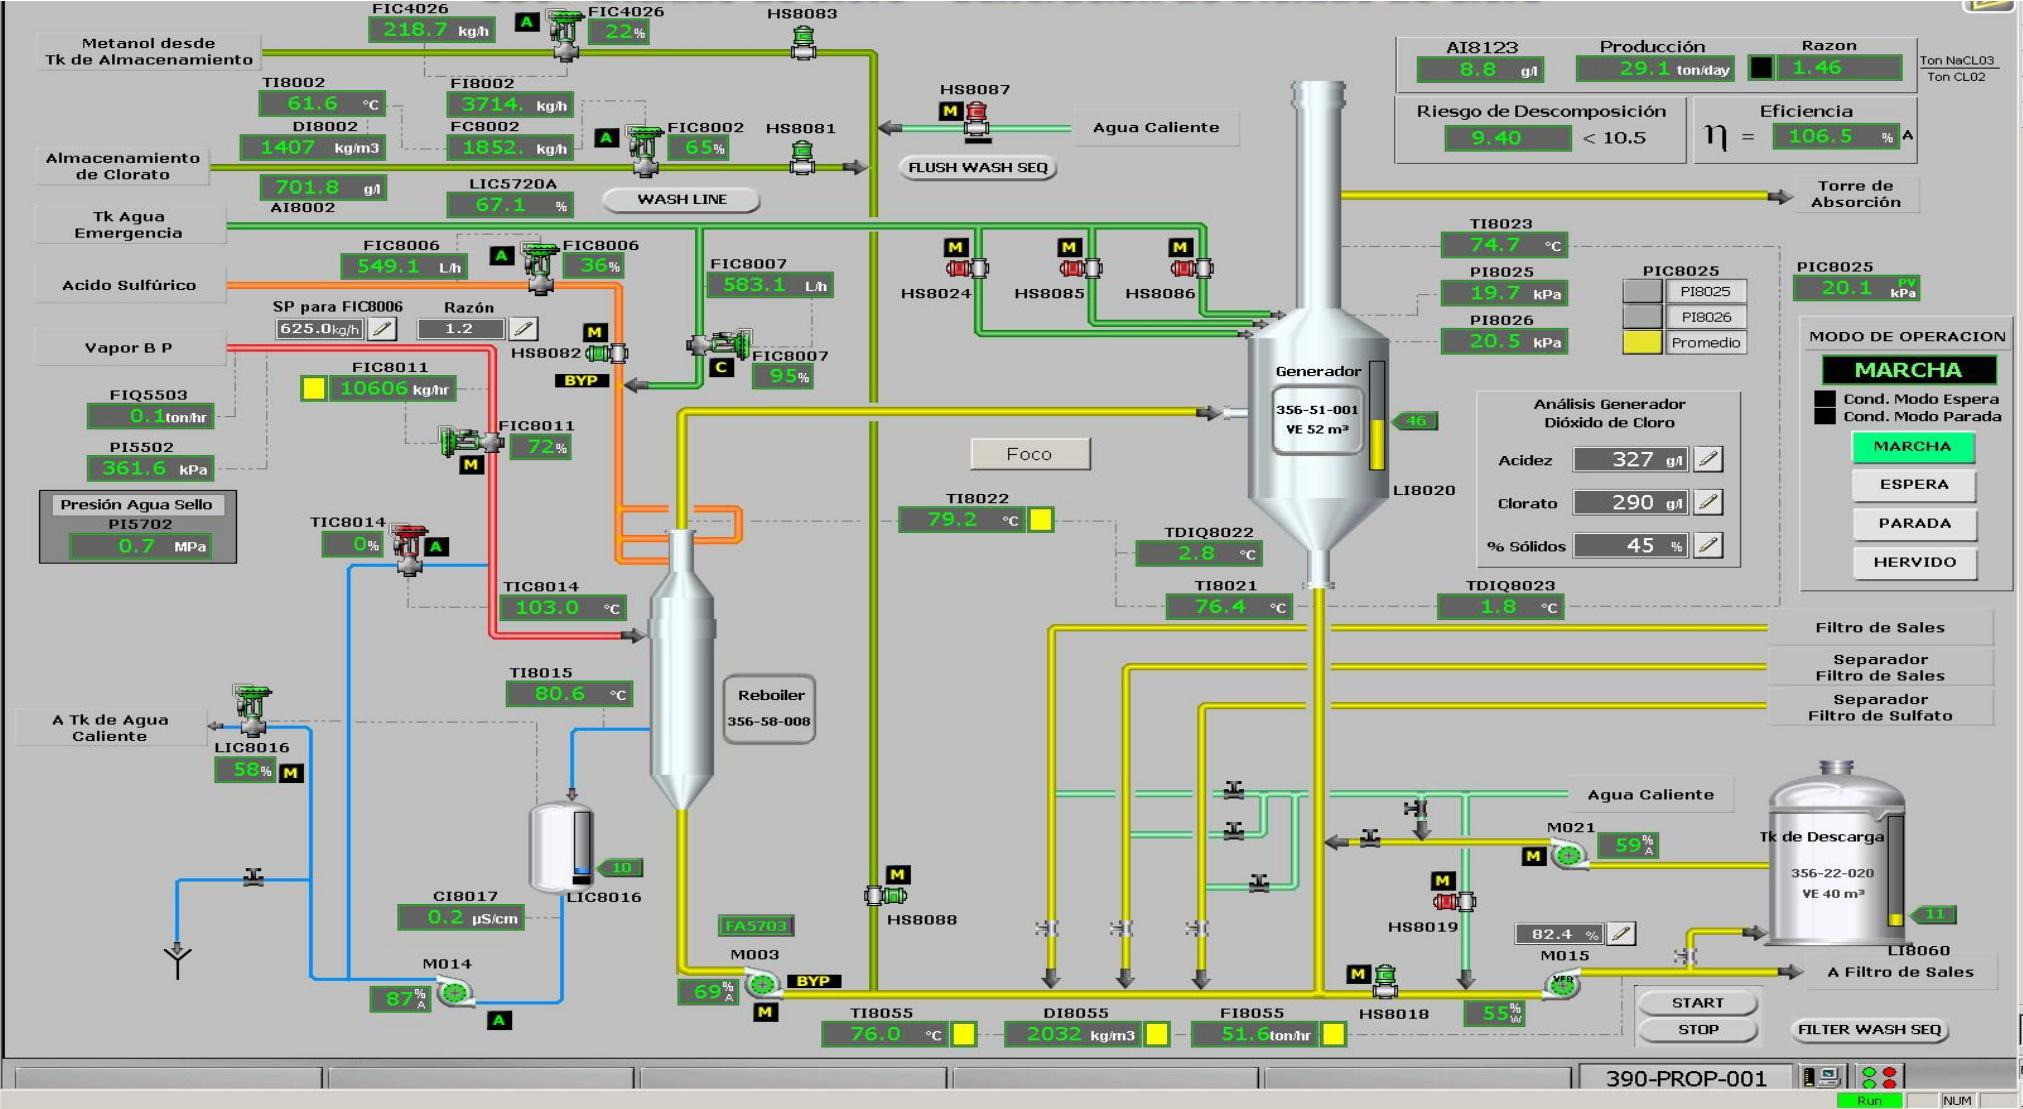
\includegraphics[width=1\linewidth]{figures/cellulose-plant.jpg}
		\caption{Schematic of the cellulose plant}
		\label{fig:cellulose-plant}
	\end{figure}

	Table \ref{tab:equipment} shows the main equipment related to the reboiler degradation.
	
	% Please add the following required packages to your document preamble:
	% \usepackage{graphicx}
	\begin{table}[pos=h]
		\centering
		\caption{Main equipment related to the reboiler degradation}
		\label{tab:equipment}
		\resizebox{\textwidth}{!}{%
			\begin{tabular}{|l|l|}
				\hline
				\textbf{Equipment}                                & \textbf{Function}                                                \\ \hline
				Generator (G)                            & Generates chlorine dioxide                              \\ \hline
				Reboiler (R) &
				\begin{tabular}[c]{@{}l@{}}Shell and tube heat exchanger. Reinjects output water of the generator as\\ vapor into the process\end{tabular} \\ \hline
				Condensate tank (CT)                     & Condensed water from the reboiler is stored here        \\ \hline
				Hot-water system reinjection pump (M014) & Reinjects the content of the CT to the hot water system \\ \hline
				Salts recuperation system reinjection pump (M015) &
				\begin{tabular}[c]{@{}l@{}}Connected to the generator, it controls the flow of sub-products from the generator such as salts, reinjecting them to\\ a salt recuperation system.\end{tabular} \\ \hline
				Pump (M003)                              & From the reboiler to tank 22-020                        \\ \hline
			\end{tabular}%
		}
	\end{table}
	
	The sulphate inlays (scaling) generated in the interior of the reboiler tubes
	(degradation) reduces the generation of chlorine dioxide, what is considered as the anomalous behaviour of the system. Figure \ref{fig:degradation} shows the degradation.
	
	\begin{figure}[h]
		\centering
		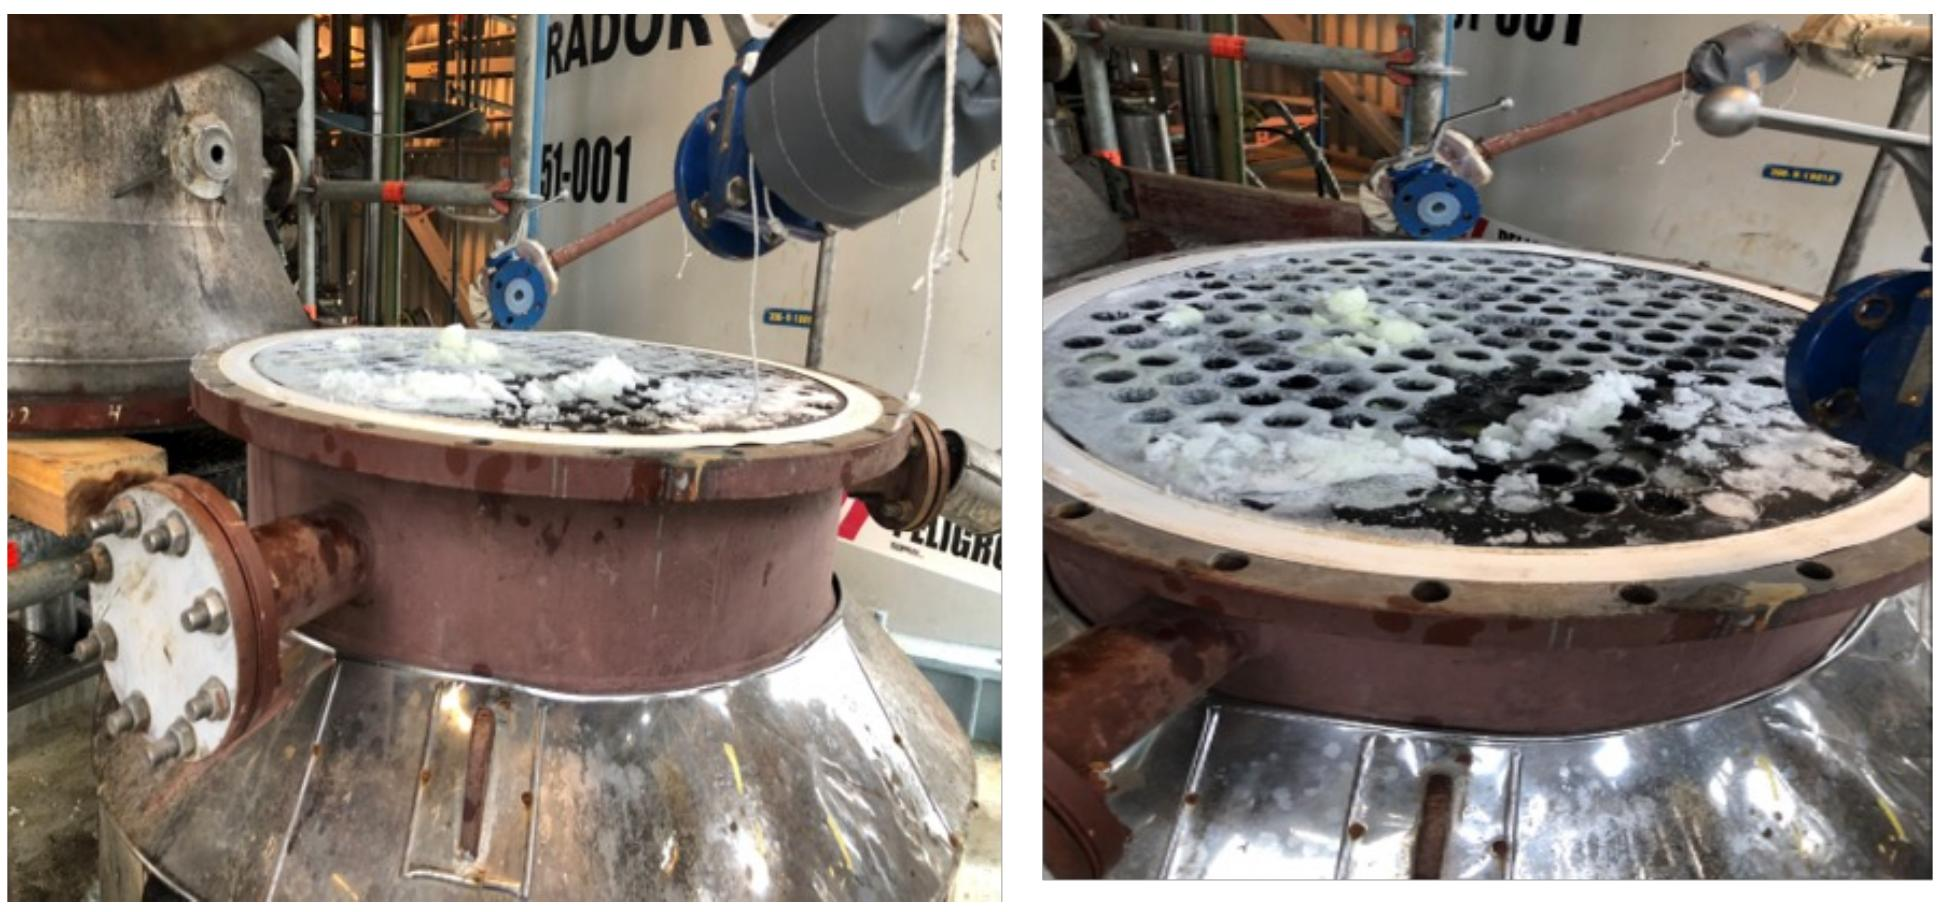
\includegraphics[width=1\linewidth]{figures/degradation.jpg}
		\caption{Sulphate inlays (scaling) generated in the interior of the reboiler tubes
			(degradation)}
		\label{fig:degradation}
	\end{figure}

	This goal of this paper is to design a neural network do diagnose faults given the information generated by the sensors that monitor the equipment involved with the reboiler. These sensors are described in Table \ref{tab:sensors}.
	
	% Please add the following required packages to your document preamble:
	% \usepackage{graphicx}
	\begin{table}[pos=h]
		\centering
		\caption{Sensors used to monitor the reboiler's condition}
		\label{tab:sensors}
		\resizebox{\textwidth}{!}{%
			\begin{tabular}{|l|l|}
				\hline
				\textbf{Sensor}                     & \textbf{Function}                                                                                                            \\ \hline
				Temperature sensor TIC8014 [$^{\circ}$C] & Measures the temperature of the water-vapor in the reboiler. High temperatures, above 110◦C indicates, an anomalous behavior \\ \hline
				Temperature sensor TI8015 [$^{\circ}$C] &
				\begin{tabular}[c]{@{}l@{}}Measures the temperature of the condensate water that goes from the reboiler to the condensate tank. High temperatures, above 110°C,\\ indicates an anomalous behavior\end{tabular} \\ \hline
				Conductivity sensor CI8017 [$\mu$S/cm] &
				\begin{tabular}[c]{@{}l@{}}Measures the conductivity of the condensed water that flows from the condensate tank to the M014 pump. Sudden conductivity\\ increments indicates an anomalous behavior\end{tabular} \\ \hline
				Pressure sensor PI8026 [kPa]    & Measures directly the pressure in the top of the generator. A sudden increase of pressure indicates an anomalous behavior    \\ \hline
				Pressure sensor PIC8025 [kPa] &
				\begin{tabular}[c]{@{}l@{}}Measures the difference of pressure in the generator from vacuum losses. A sudden increase of differences of pressure indicates an\\ anomalous behavior\end{tabular} \\ \hline
				Power of the M014 pump [\%]     & Measures the power load on the hot-water system reinjection pump. A high-power load indicates an anomalous behavior          \\ \hline
				Power of the M015 pump {[}\%{]}     & Measures the power load on the salts recuperation system reinjection pump. A high-power load indicates an anomalous behavior \\ \hline
				Power of the M003 pump [\%]  & -                                                                                                                            \\ \hline 
			\end{tabular}%
		}
	\end{table}

	The dataset comprises 41,539 rows (time steps with sampling frequency of 2 hours) and 10 columns, where columns 2 to 9 correspond to the sensors readings and the last one the reboiler’s health states (0 for normal behaviour and 1 for anomalous behaviour).

	\section{Data Preprocessing and Neural Network Design}\label{sec:nn-design}
	Before designing the neural network, a preliminary analysis was performed on the available dataset, from which it was observed that there were missing data in some rows, and that the dataset was not normalized, as shown in the histogram in Figure \ref{fig:histogram}. To solve this issue, a data transformation pipeline was applied to fill in the missing values with the column average, and also normalize the values of each column between 0 and 1.
	
	\begin{figure}[h]
		\centering
		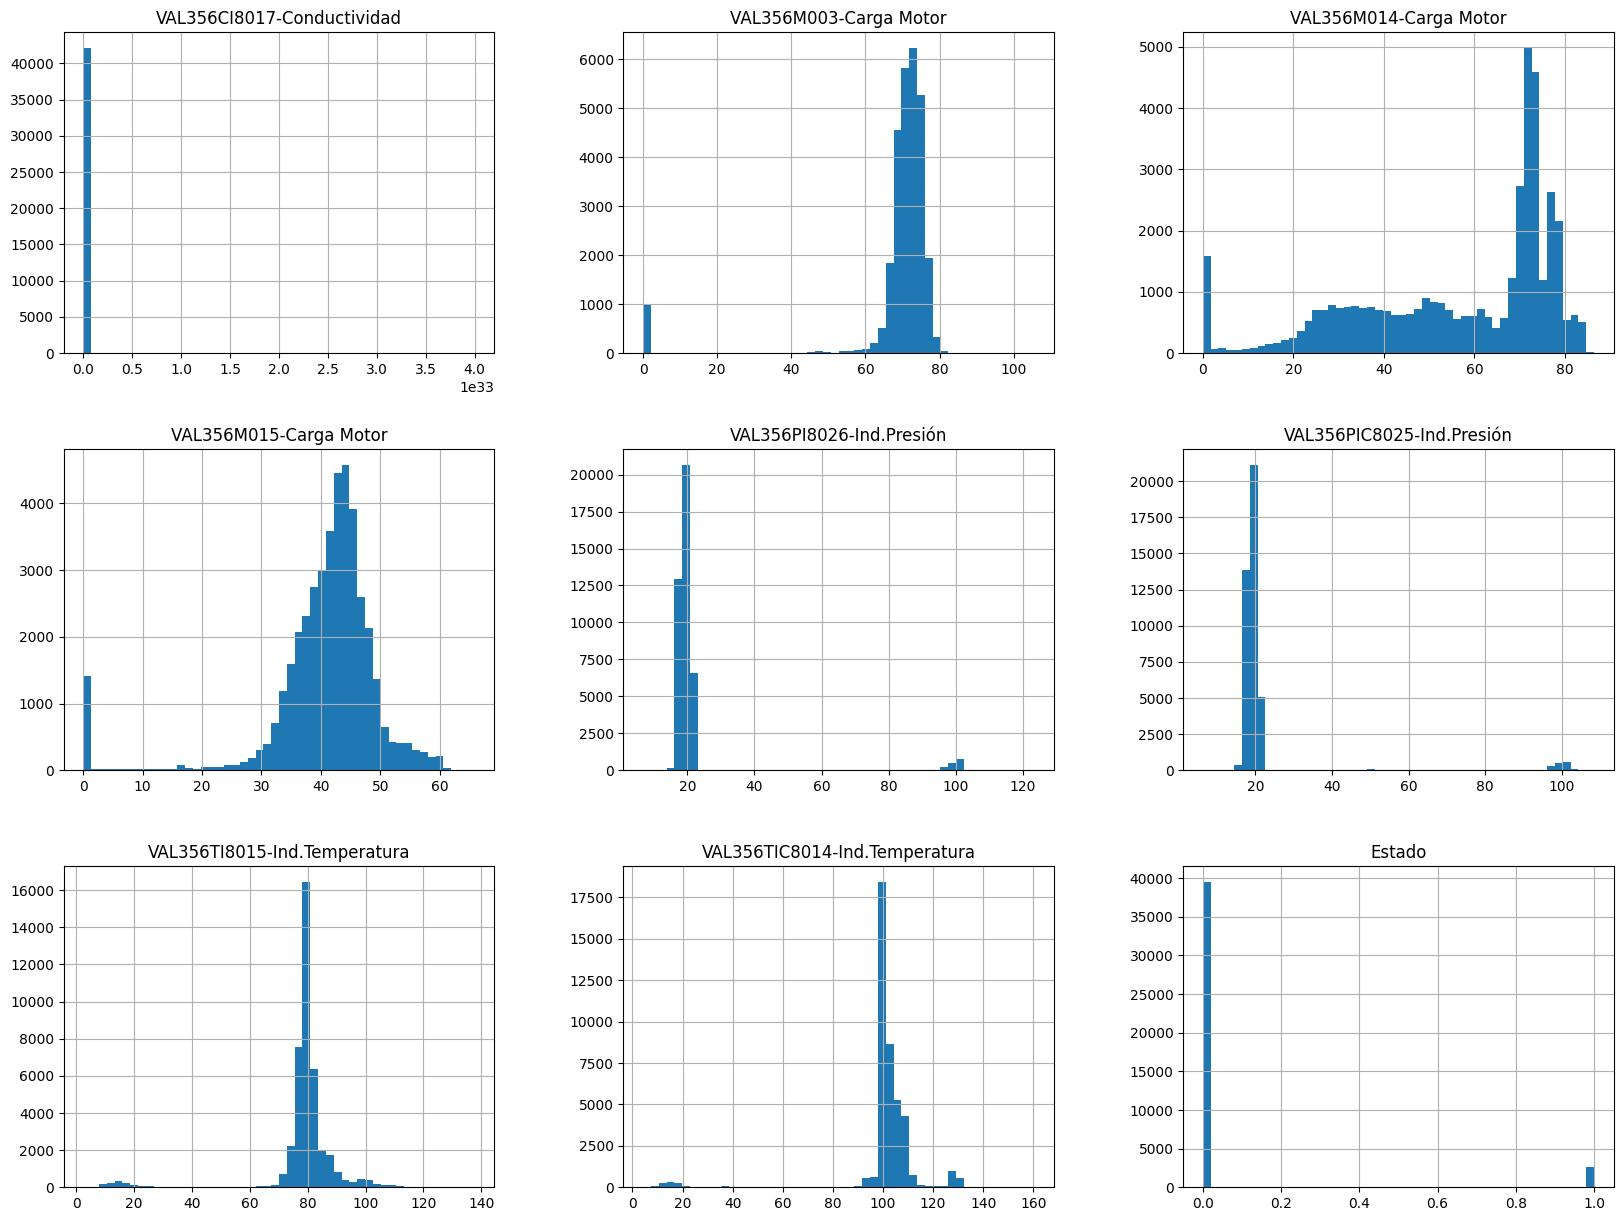
\includegraphics[width=1\linewidth]{figures/histogram.jpg}
		\caption{Histogram of the features and label}
		\label{fig:histogram}
	\end{figure}	

	The next step was then to shuffle and split the dataset, which resulted in 27,011 instances for training, 6,753 for validation, and 8,442 for testing. Then, a fully connected multilayer perceptron (MLP) neural network model was created for training: 8-dimensional input vector, followed by hidden layer with 32 neurons and sigmoid activation function, and output layer with 2 neurons and softmax activation. The model was compiled with sparse crossentropy categorical loss, adam optimizer and accuracy as metric. Training was designed to be done in 100 epochs using the early stopping callback, which would stop training as long as there was no improvement in validation loss for 10 consecutive epochs.
	
	\section{Results}\label{sec:results}
	
	The learning curves are shown in Figure \ref{fig:learning-curves}. The early stopping callback was not triggered because there was no increase in validation loss during training for more than 10 consecutive epochs. The weights used in the final model were those of the 100th epoch, which presented the lowest validation error (0.0134).
	
	\begin{figure*}[h]
		\centering
		\begin{subfigure}[b]{0.8\linewidth}
			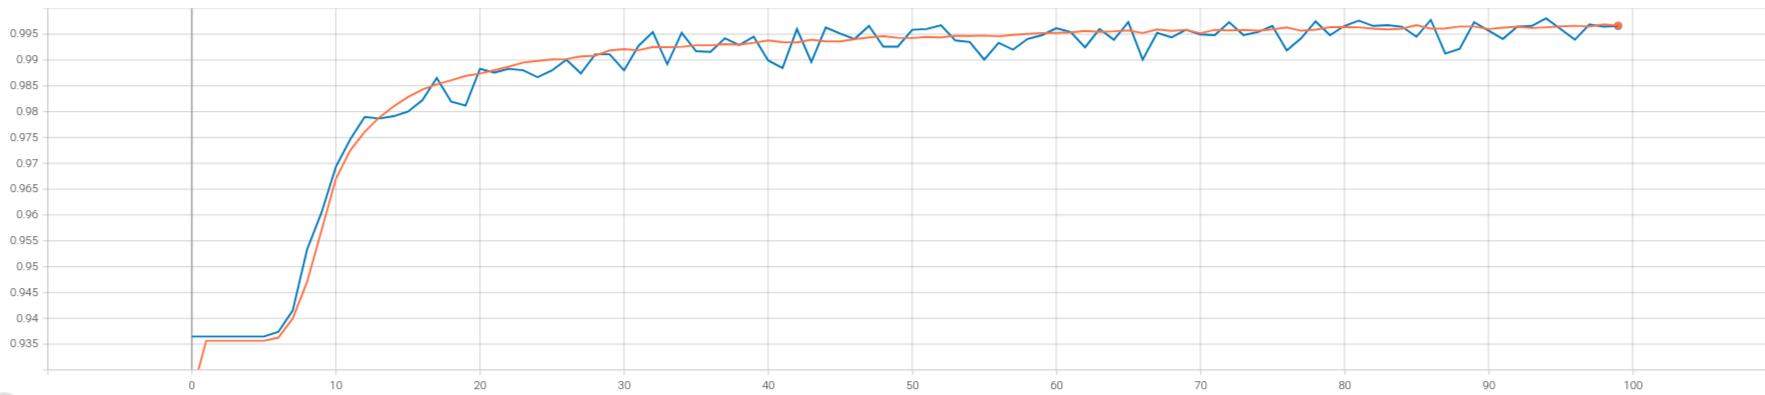
\includegraphics[width=1\linewidth]{figures/accuracy-big.jpg}
			\caption{Accuracy per epoch}
			\label{fig:accuracy}
		\end{subfigure}
		\begin{subfigure}[b]{0.8\linewidth}
			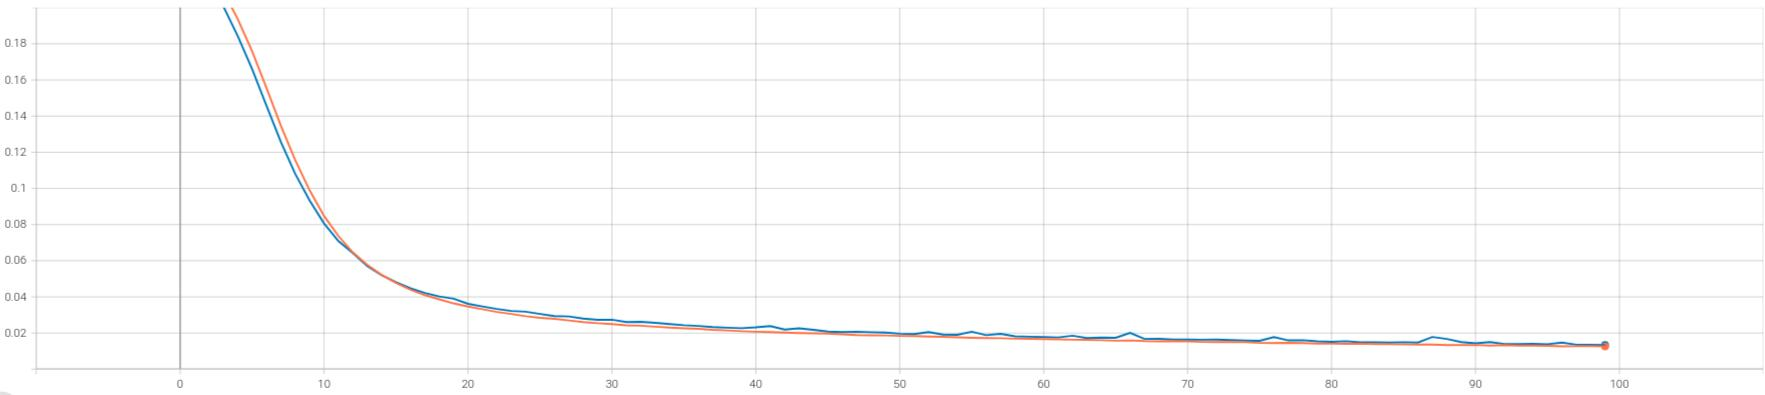
\includegraphics[width=\linewidth]{figures/loss-big.jpg}
			\caption{Loss per epoch}
			\label{fig:loss}
		\end{subfigure}
		\caption{Learning curves: training (orange) and validation (blue)}
		\label{fig:learning-curves}
	\end{figure*}
	
	Figure \ref{fig:evaluation-test-set} shows the model's confusion matrix and ROC curve over the test data. The calculated accuracy was 99.61\%, while the area under the ROC (Receiving Operating Characteristic) curve was 99.98\% (from a maximum of 100\% for a perfect classifier). The curve of a random classifier is also plotted, which has a 50\% chance of getting the class of each new instance right.
	
	\begin{figure*}[h]
		\centering
		\begin{subfigure}[b]{0.45\linewidth}
			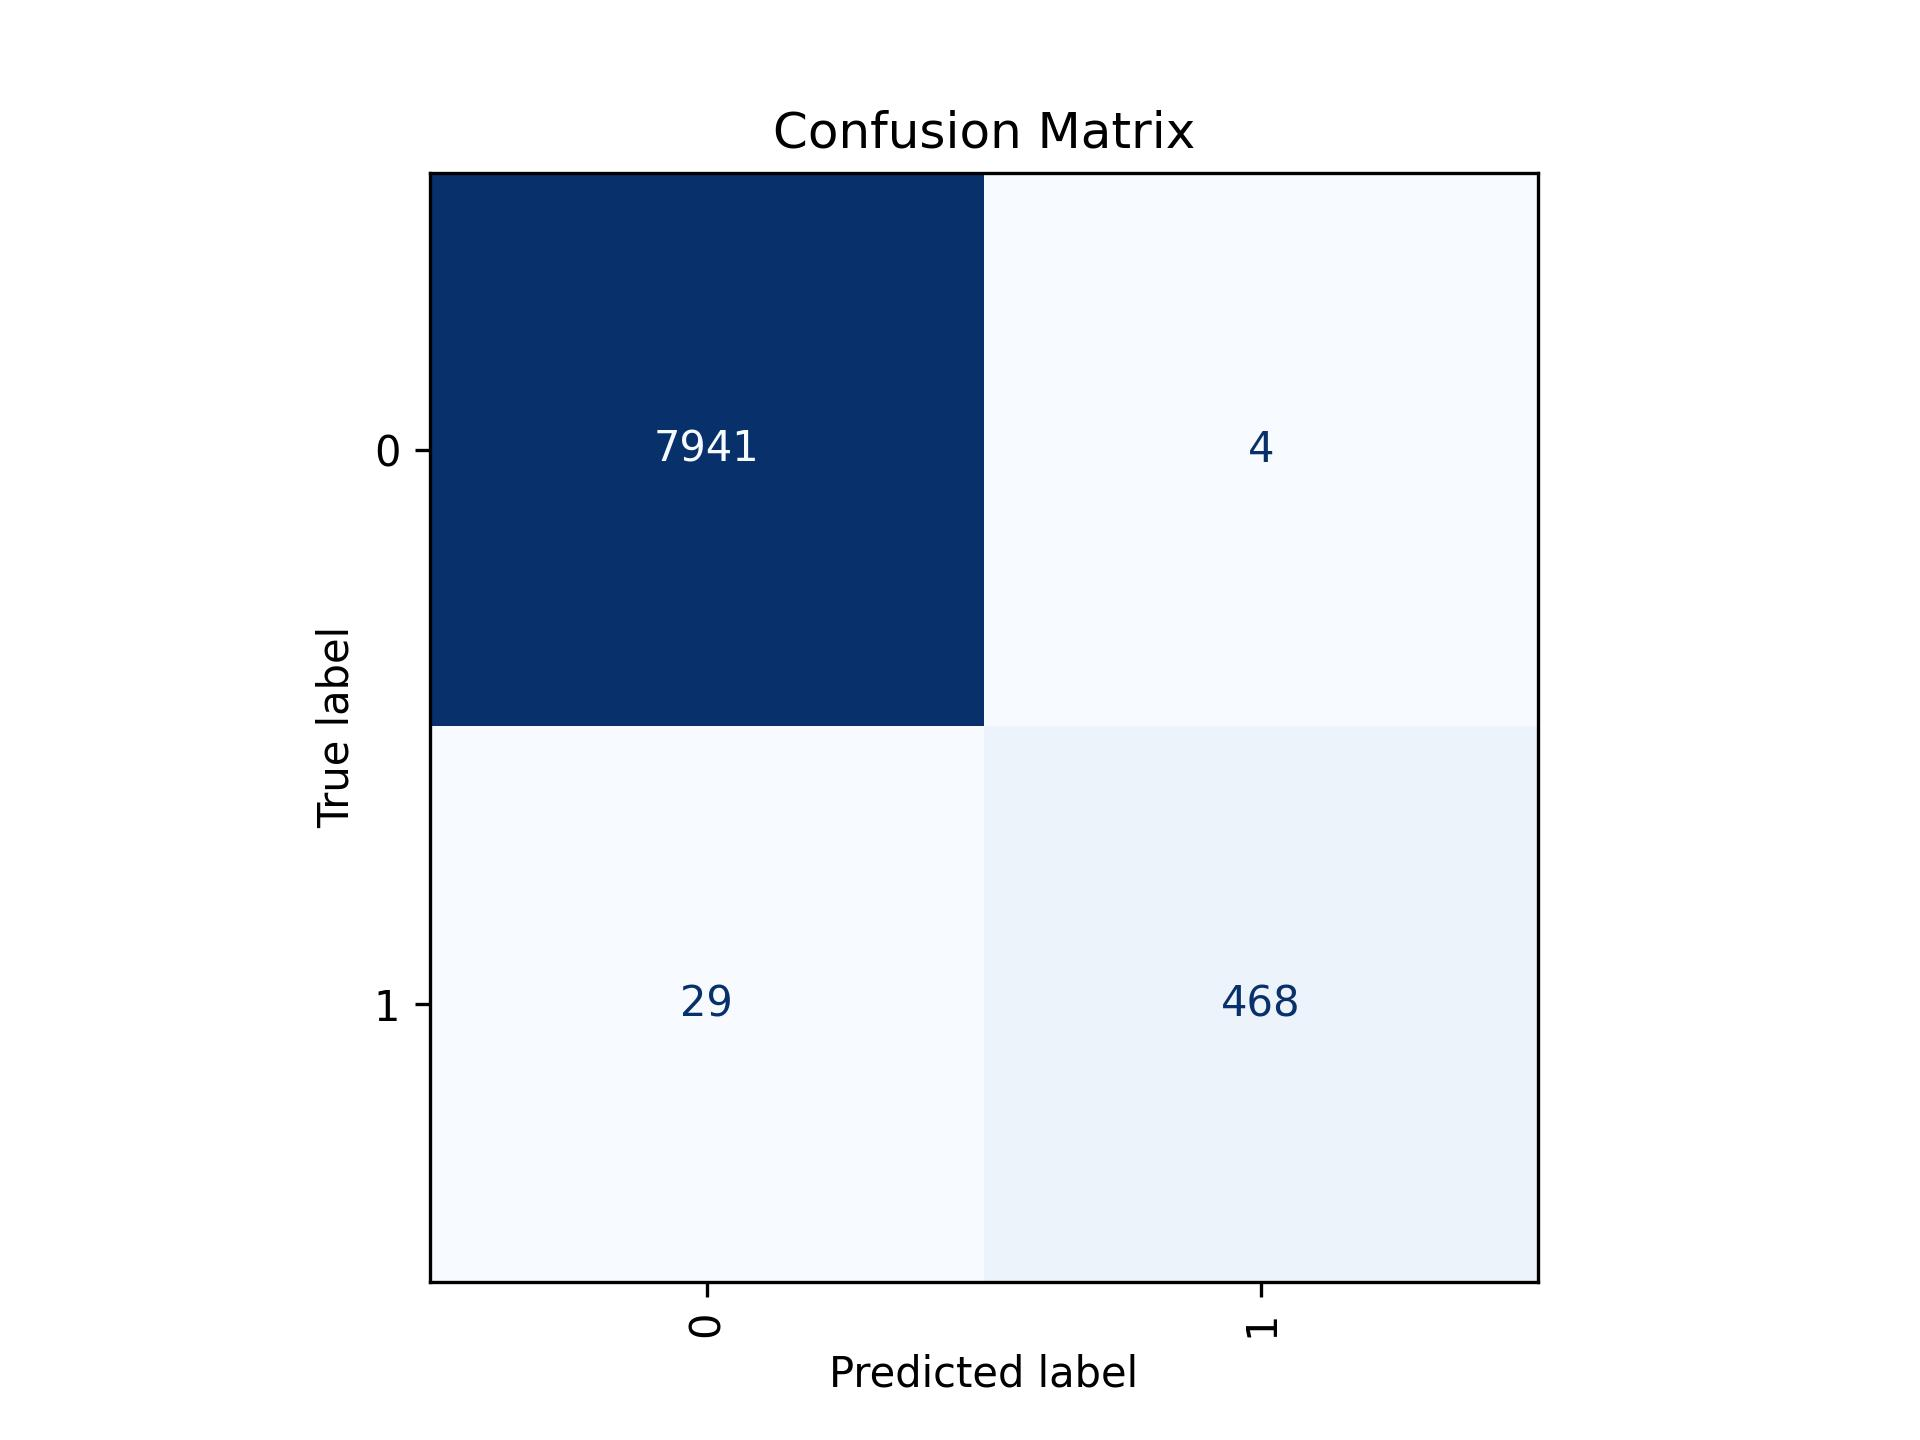
\includegraphics[width=1\linewidth]{figures/confusion-matrix.jpg}
			\caption{Confusion Matrix}
			\label{fig:confusion-matrix}
		\end{subfigure}
		\begin{subfigure}[b]{0.45\linewidth}
			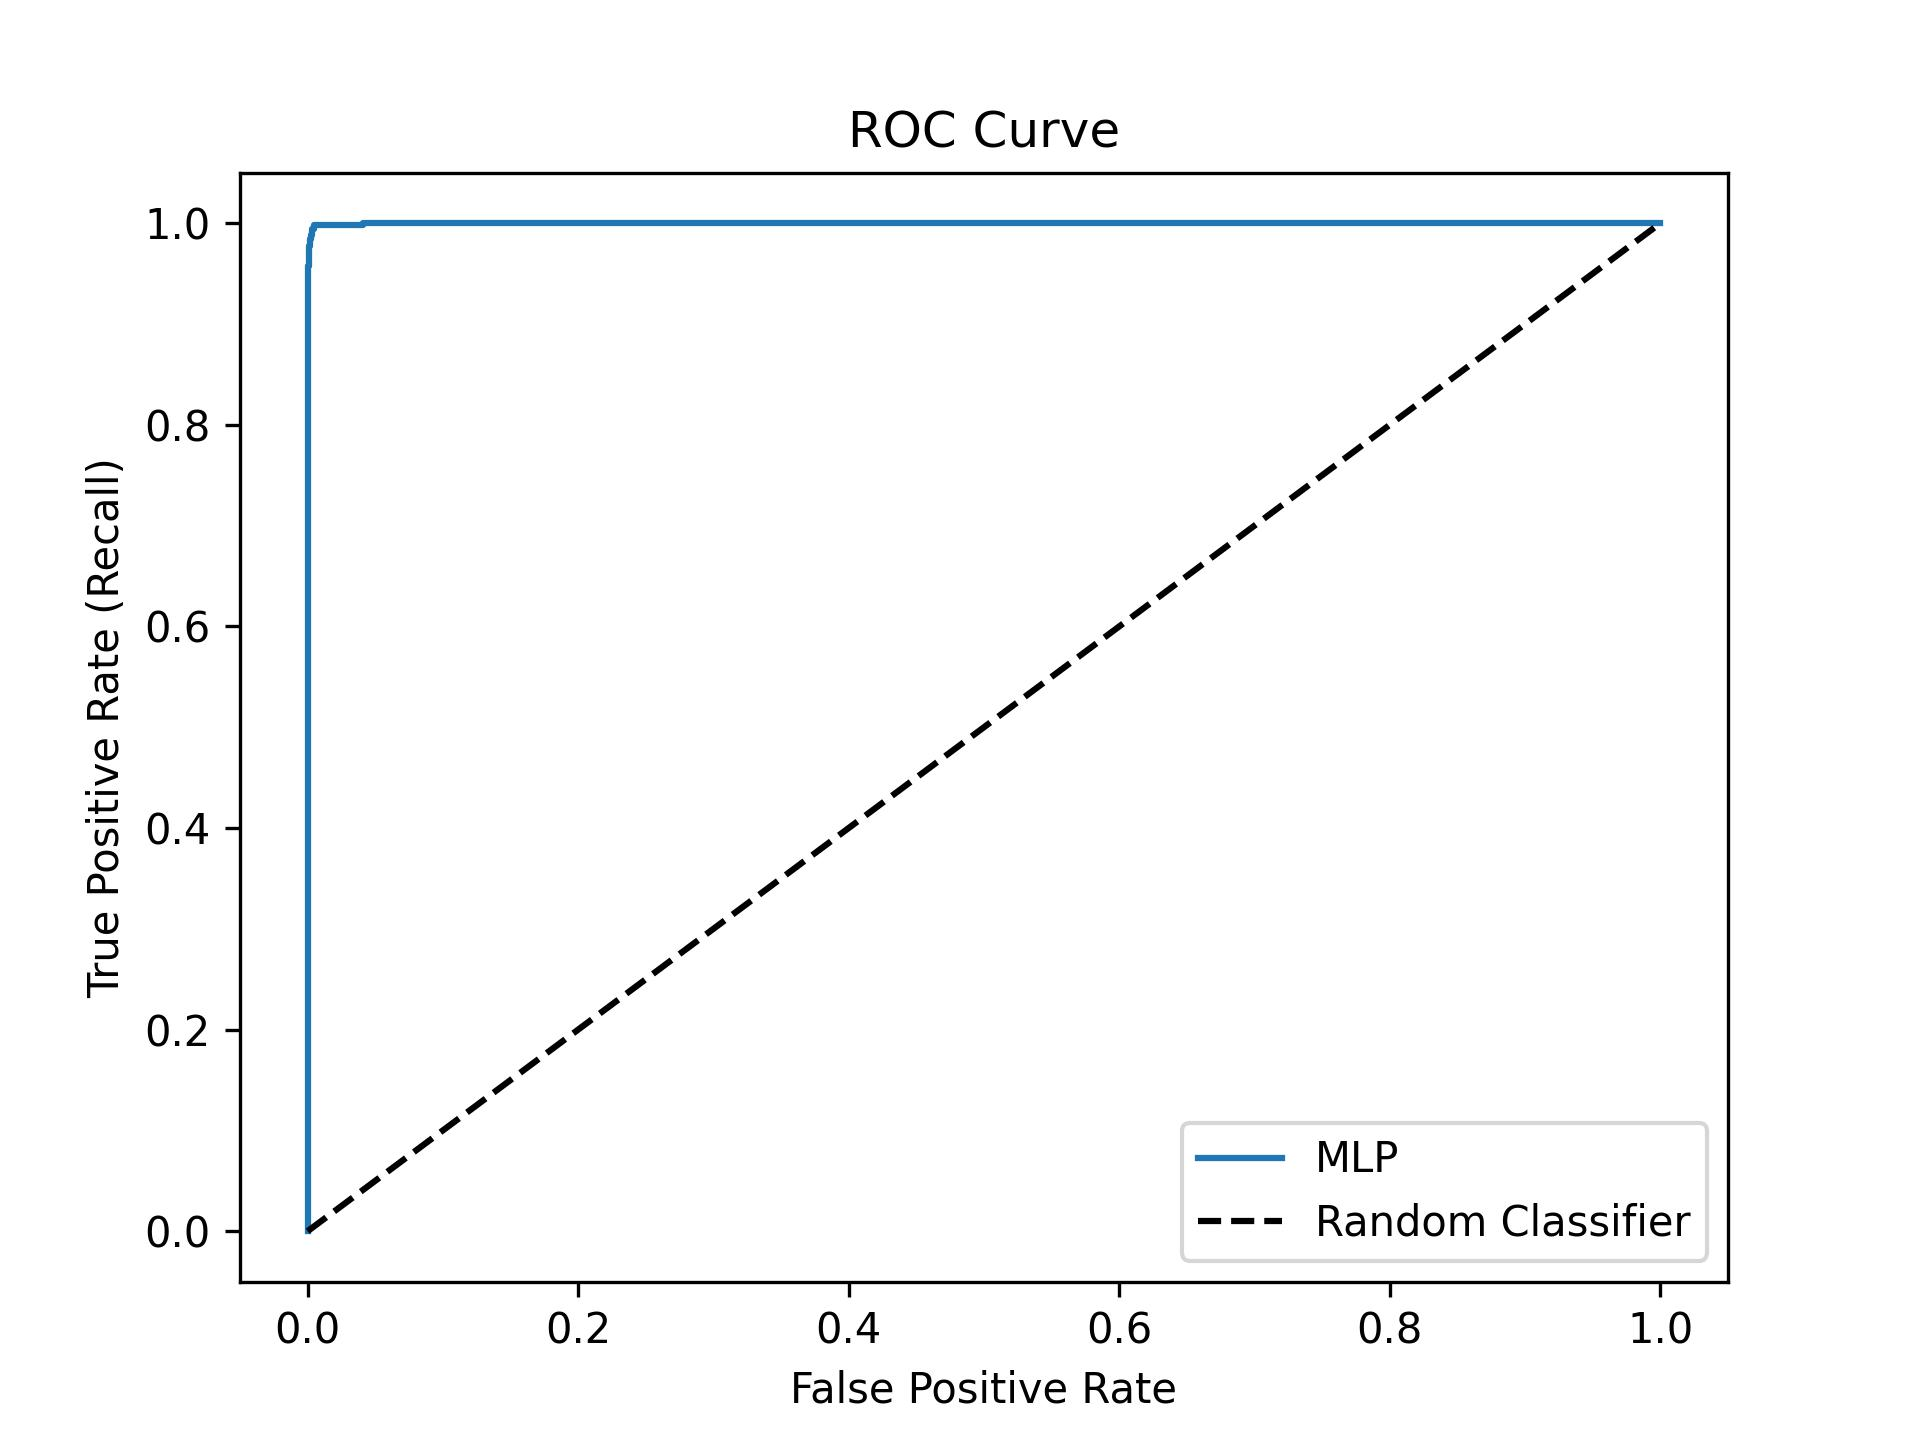
\includegraphics[width=\linewidth]{figures/roc-curve.jpg}
			\caption{ROC Curve}
			\label{fig:roc-curve}
		\end{subfigure}
		\caption{Evaluation on test set}
		\label{fig:evaluation-test-set}
	\end{figure*}
	
	
	\section{Conclusions}\label{sec:conclusion}
	
	Preprocessing a dataset containing 41,539 instances of data from 8 sensors relevant to a reboiler to fill missing values and normalize the values between 0 and 1, and using an MLP neural network with 2 layers -- a hidden one with 32 neurons and sigmoid activation, and an output one with 2 neurons with softmax activation -- , adam optimizer, sparse categorical crossentropy as loss, accuracy as a metric, and training the model for 100 epochs, it was possible to classify the health status of the equipment (0 for healthy and 1 for anomalous behavior) with an accuracy of 99.61\% and area under the ROC curve of 99.98\%. The classifier proved to be promising to be used as a tool for monitoring the condition of the equipment.
		
	% To print the credit authorship contribution details
%	\printcredits
	
%	\section*{Declaration of competing interest}
%	The authors declare that they have no known competing financial interests or personal relationships that could have appeared to influence the work reported in this paper. 
	
	%% Loading bibliography style file
	\bibliographystyle{model1-num-names}
	%\bibliographystyle{cas-model2-names}
	
	% Loading bibliography database
%	\bibliography{references}
	
	%% Biography
	%\bio{}
	%% Here goes the biography details.
	%\endbio
	%
	%\bio{pic1}
	%% Here goes the biography details.
	%\endbio
	
\end{document}

